\chapter{Directional Noise Elimination}\label{ch:directional}
\section{Introduction}
This chapter deals with directional filtering. The idea is presented and tested. The 
results and conclusions will be shown afterwards.
\section{Concept}
Figure \ref{fig:2sources} shows a scenario where directional filtering could be used.
Source 1 and Source 2 are both talking simultaneously. At the Origin, two microphones 
left(L) and right(R) are recording both signals.

\begin{figure}[htp]
	\centering
	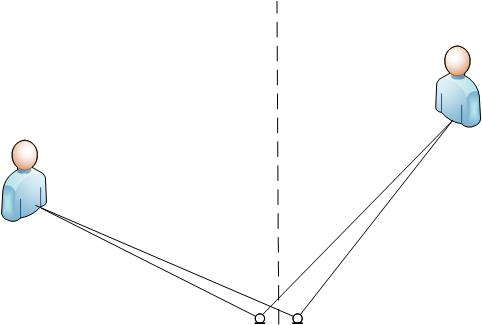
\includegraphics[width=0.8\textwidth]{Illustrations/2sources.jpg}
	\caption{Two Persons Talking}
	\label{fig:2sources}
\end{figure}

Due to the placement of the sources, both microphones will record the sounds, with a 
certain delay.
\section{Development}
\section{Conclusion}